%% YT-Diag --- DLDM final report
%%
%% SINGLE-FILE ON PURPOSE. The AAAI style forbids \input: "Your LaTeX source
%% file (excluding references) must consist of a single file (use of the
%% `input' command is not allowed)" (AAAI_formatting_reference.tex, l.71/81).
%% So do NOT split this into sections/*.tex -- it would not be submittable.
%% Navigate with the %% ==== banners instead.
%%
%% Other AAAI hard requirements, all already satisfied below:
%%   two-column aaai.sty, letterpaper, Times (not Computer Modern),
%%   no page numbers / headers / footers, no embedded links (so no hyperref),
%%   PDFLaTeX only (no .eps figures), bibliography via aaai.bst.
%%
%% DRAFT MARKERS: \note{STATUS}{text} renders only while \drafttrue. Flip to
%% \draftfalse before submission and every marker disappears at once.
%%   CONFIRMED      reproduced from code output; source named in claim_evidence.md
%%   PROVISIONAL    a decision we have made but not yet team-signed-off
%%   PENDING        awaiting an experiment that has not run
%%   LIMITATION     known threat to validity, must survive into the final text
%%   SIGNOFF        Emmanuel + Adam must decide
%%
%% Numbers must never be typed by hand. make_tables.py rewrites the region
%% between the <<<BEGIN GENERATED ...>>> markers from the saved results.json
%% files -- in place, so the single-file rule still holds. Regenerate, do not
%% edit inside a generated block.

\documentclass[letterpaper]{article}
\usepackage{aaai}
\usepackage{times}
\usepackage{helvet}
\usepackage{courier}
\usepackage{amsmath}
\usepackage{graphicx}
\usepackage{booktabs}
\usepackage{xcolor}
\frenchspacing
\setlength{\pdfpagewidth}{8.5in}
\setlength{\pdfpageheight}{11in}
\setcounter{secnumdepth}{0}

\newif\ifdraft\drafttrue          % <-- \draftfalse before submission
\newcommand{\note}[2]{\ifdraft{\small\textcolor{red}{[\textbf{#1}: #2]}}\fi}

\pdfinfo{
/Title (YT-Diag: Predicting and Explaining Within-Niche YouTube Video Performance)
/Author (Adam Michalik, Emmanuel Gyabaah)}

\begin{document}

\title{YT-Diag: Predicting and Explaining\\Within-Niche YouTube Video Performance}
\author{Adam Michalik \and Emmanuel Gyabaah\\
Technical University of Munich\\
Deep Learning and Decision Making\\
\{go54lix, emmanuel.gyabaah\}@tum.de}
\maketitle

\begin{abstract}
\begin{quote}
Creators are told that thumbnails, pacing and titles drive video performance,
but such advice is rarely measured against the variables that actually dominate
outcomes. Predicting raw view counts is largely a channel-size readout: we show
that a model given only subscriber count, video age, duration and video format
--- with no access to content --- reaches an out-of-fold $R^2$ of 0.584 on
$\log(1+\mathrm{views})$. Existing engagement work either predicts absolute
popularity, which inherits this confound, or relies on watch-time signals that
the public API does not expose. We therefore reformulate the task: rather than
predicting views, we predict whether a video ranks in the top quarter of a peer
group matched on category, channel size, video age and format, and we report the
non-content baseline explicitly so that any content result is read against it.
We assemble two cohorts --- a retrospective multimodal archive of 1,860 videos
and a prospective panel of 12,738 videos as of 2 September, with twice-daily outcome tracking
--- and map both onto a single feature table so that every ablation is a choice
of feature groups rather than a separate pipeline. On the resulting label,
after nested selection, metadata+schedule XGBoost reaches validation AUC
$0.619\pm0.022$, while our best frozen field-aware text, thumbnail and metadata
fusion reaches $0.600\pm0.026$ and the tuned full engineered baseline reaches
$0.614\pm0.023$ over five channel-grouped seeds; the test set remains sealed. Engineered vision alone
performs at chance. We show why this is a design success rather than a failure
of vision: before video format was stratified out of the label, thumbnail
brightness was detecting the composition of vertical videos rather than
content quality.
\end{quote}
\end{abstract}

%% ==================================================================
\section{Introduction}
%% ==================================================================

Creators receive abundant advice about thumbnails, pacing and titles, but little
of it is measured against the confounds that dominate video performance. A video
from a large channel outperforms a video from a small one almost regardless of
its content, so any model trained to predict raw view counts learns channel size
rather than craft.

We ask a narrower and more answerable question: \emph{within a peer group of
comparable channels, does the content of a video predict whether it performs in
the top quarter of that group, and which content features are associated with
underperformance?}

Our contributions are:
\begin{itemize}
\item A two-cohort dataset design pairing a retrospective multimodal archive
      with a live prospective panel that records fixed-horizon outcomes and
      near-publication metadata.
\item An explicit measurement of the \emph{shortcut ceiling}: how much of the
      outcome is predictable from non-content variables alone. We argue this
      figure should be reported before any modelling result.
\item A label design that neutralises the three confounds we measured --- channel
      size, video age and video format --- and evidence that failing to
      neutralise format alone produces an apparent visual signal that is really
      aspect-ratio detection.
\end{itemize}

%% ==================================================================
\section{Related Work}
%% ==================================================================

\subsection{Predicting video performance}
\textbf{Engagement prediction.} \cite{wu2018beyond} define relative engagement,
calibrating watch percentage against duration at a fixed horizon, and provide
content and channel baselines. We borrow the calibrate-by-ranking-within-strata
method only; we cannot compute their metric because watch time is not available
through the public API. Cite as ``inspired by'', never ``following''.

\subsection{Multimodal representation}
\textbf{Frame-level video features.} \cite{abu2016youtube} establish
frame-level features aggregated temporally for large-scale video classification.
\cite{rajaram2020unboxing} apply an attention-based approach to influencer video
engagement, which motivates our attribution layer.

%% ==================================================================
\section{Methodology}
%% ==================================================================

\begin{figure*}[t]
\centering
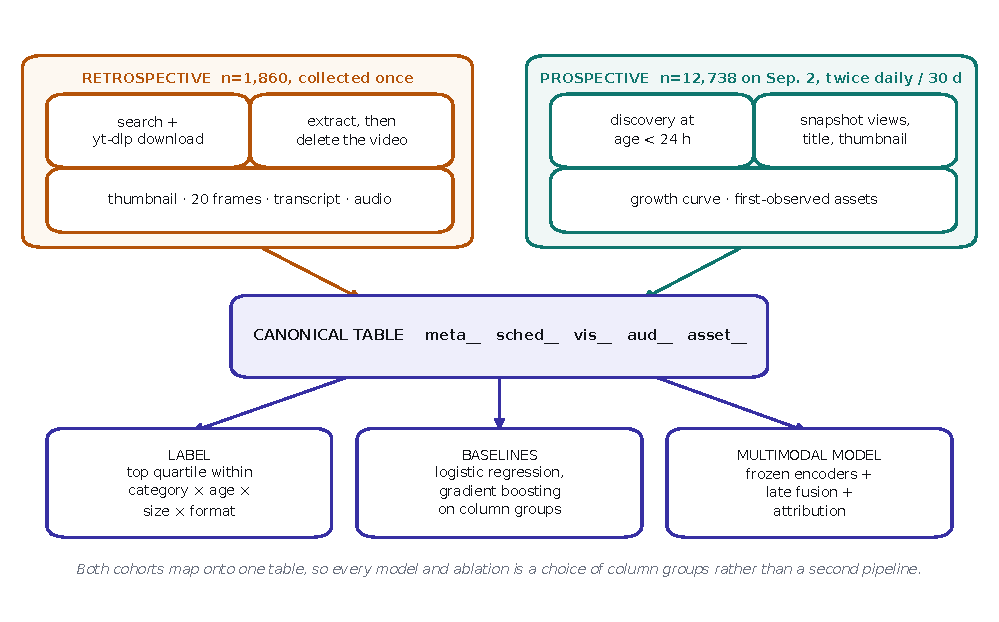
\includegraphics[width=0.86\textwidth]{figures/pipeline.pdf}
\caption{Both cohorts are mapped onto one canonical feature table, so every
model and ablation is a selection of column groups rather than a separate
pipeline. The retrospective cohort is the only source of frames, transcripts
and audio; the prospective panel is the only source of growth curves and
first-observed (pre-edit) titles and thumbnails.}
\label{fig:pipeline}
\end{figure*}

Figure~\ref{fig:pipeline} gives the overall pipeline.

\subsection{The shortcut ceiling}

Before defining a target we measured how much of it is obtainable without
looking at content. A gradient-boosted model given only subscriber count, video
age, duration and Shorts status predicts $\log(1+\text{views})$ at an
out-of-fold $R^2$ of \textbf{0.584} under channel-grouped cross-validation
(0.643 under random folds, which is the leaky comparison, not ours).

Two caveats matter for how this number is read. The folds are grouped by
channel, so it is not inflated by channel memorisation --- a random-fold split
gives a higher 0.643. But subscriber count is observed \emph{retrospectively},
after the videos accumulated their views, and a successful video raises its own
channel's subscriber count. This is therefore a diagnostic of how much of the
outcome is explained by non-content variables in our data, not a leakage-free
prospective estimate. The prospective cohort exists partly to remove exactly
this circularity, by recording subscriber count near publication.

We therefore make two commitments. Raw view count is never our modelling target,
and no $R^2$ on views is reported as evidence of content signal.
\note{CONFIRMED}{02\_Data/eda\_retrospective.py::shortcut\_ceiling}

\subsection{Label}

A video is labelled \emph{viral} if it falls in the top quarter of its cell,
where a cell is the intersection of category, an age band, a channel-size band
and video format. Bands are equal-count quantile bands assigned \emph{by value},
so videos with identical (API-rounded) subscriber counts can never be split
across bands, and are computed \emph{within} a format stratum. The configuration
is $3\times3\times2$ per category, giving 1{,}854 labelled videos and a 23.6\%
positive rate.

Formally, let $c(v)$ denote the cell of video $v$, defined by the tuple
(category, age band, channel-size band, format). Within each cell we rank by
$s(v) = \log(1 + \mathrm{views}(v))$ and label

\begin{equation}
\begin{split}
k_c &= \max\!\left(1,\; \lfloor 0.25\,|c| \rfloor\right), \\[2pt]
y(v) &= \mathbf{1}\!\left[\, \mathrm{rank}_{c(v)}\big(s(v)\big) > |c(v)| - k_{c(v)} \right],
\end{split}
\end{equation}

\noindent so exactly $k_c$ videos in each cell of size $|c|$ are positive. The $\log$ is monotone and therefore does not change
the within-cell ranking; it is retained because the stored score is also a
readable quantity for analysis. Bands are equal-count quantile bands assigned
\emph{by value}, so videos sharing an (API-rounded) subscriber count can never
fall in different size bands.

Three design choices departed from our initial plan, each on measured evidence:

\textbf{No minimum-age floor.} Our first design excluded videos under 30 days
old, inherited from a views-per-day formulation that decays with age. Ranking
within age bands does not share that problem, and the floor cost 861 videos
(46\%, and a biased 46\%: 64\% Shorts against 43\% retained) while changing the
four-confound label AUC only from 0.576 to 0.572. We tested its premise directly
on the prospective panel, the only place a video is observed at two ages: view
\emph{rank} is roughly 90\% settled within 24 hours (day-1 to day-5 Spearman
0.946), while the raw count still doubles --- which is exactly why the label must
remain a within-band ranking rather than a count threshold.
\note{LIMITATION}{Measured to day 5 only; the panel is not yet old enough to
confirm stability to day 30. Re-check after 2026-09-25.}

\textbf{Format as a stratifier.} Unstratified, Shorts take the viral label at
roughly twice their population share, and the label becomes predictable from
format alone at AUC 0.596. Stratifying reduces that to 0.447.

\textbf{Three bands, not four.} Adding the format dimension halves every cell, so
$4\times4\times2$ leaves a median cell of 13 with 102 cells below our
small-cell threshold, while $2\times2\times2$ readmits the confounds (AUC 0.660).
\note{SIGNOFF}{Adam to confirm all three; they revise the label definition
locked in the proposal.}

\subsection{Format leakage}

Video format is not something a model must infer: portrait framing recovers it
for 99.0\% of videos, while raw thumbnail brightness predicts it at
direction-free AUC 0.925, largely because vertical source imagery is often
padded or composed differently inside a 16:9 thumbnail. A heuristic content
crop reduces this to 0.559, but is not a verified pillarbox detector.
Stratifying the label prevents format from inflating a score, and we report a
format-only baseline alongside every visual result.

\subsection{Evaluation protocol}

Splits are channel-grouped 60/20/20 via stratified group $k$-fold; no channel
appears in two splits, and this is asserted at runtime. The grouping is
load-bearing: predicting the label from channel-level features alone reaches AUC
0.644 under random folds. The test split is evaluated exactly once, at the end.
\note{LIMITATION}{Per-category test sets are too small for per-category claims:
roughly 6--7 positives per category per split. We report pooled metrics with
spreads and treat per-category numbers as descriptive only.}

\subsection{Frozen multimodal model}

We first test the smallest deep model that can establish whether raw content
adds value. A revision-pinned DINOv2 ViT-S/14 maps the 224-pixel centre crop of
each thumbnail to its frozen 384-dimensional class token. A revision-pinned
ModernBERT-base maps the title, cleaned transcript and description (in that
priority order under a 1{,}024-token cap) to a frozen 768-dimensional
attention-mask-weighted mean. Separate presence masks distinguish missing
transcripts or descriptions from measured zeros. The cleaning manifest exposes
only 1{,}404 transcripts as usable; the remaining 456 sparse or wrong-language
transcripts are withheld while their title and description remain.

We evaluate both an L2 logistic probe and a late-fusion MLP. The MLP projects
each modality to 32 dimensions, concatenates the projections, and applies a
32-unit head with GELU and 0.5 dropout. Logistic regularisation and the MLP
epoch are selected on a channel-grouped split wholly inside the training fold;
the selected model is refitted on the outer training fold before validation.
The encoders never train. Frames are deliberately deferred until this cheaper
thumbnail/text stage demonstrates stable added value.

The generic representation is followed by one targeted text experiment. An
embedding-trained ModernBERT variant encodes title, description and transcript
separately, using the model's document prefix and masked-mean pooling. Long
transcripts contribute up to four evenly distributed, overlapping 384-token
chunks rather than only their opening; field and chunk embeddings are
L2-normalised and reduced to the model's 256-dimensional Matryoshka
representation. This policy is fixed before the five-seed run and the encoder
remains frozen.

%% ==================================================================
\section{Experiment}

%% ==================================================================

\subsection{Dataset}

\textbf{Retrospective archive.} 1{,}860 already-published videos across four
categories (comedy 464, how-to 373, product reviews 482, vlogs 541), collected
once in August 2026 from 1{,}319 distinct channels. Each video contributes
metadata, a thumbnail, 20 sampled frames, a transcript, and engineered visual and
audio features. This is the only cohort carrying full content modalities and is
therefore what the multimodal model trains on.
\note{LIMITATION}{Short of the 8{,}000 target: search.list pagination caps out
well below its advertised result counts. Same limit the CC-availability scan hit.}

\textbf{Prospective panel.} A live cohort of newly published videos discovered
daily and snapshotted twice daily for 30 days, 11{,}256 videos at time of
writing. It carries growth curves and, critically, the \emph{first-observed}
title and thumbnail --- before creators edit them --- which the retrospective
archive can never recover.
\note{LIMITATION}{Its 30-day outcomes mature after this submission, so it is
reported here as design and future work, not as results. Feature availability is
two-phase: content modalities are extracted only for a sample selected after the
cohort is frozen at the horizon.}

Frames are sampled non-uniformly: 12 of 20 fall inside the first 60 seconds,
because retention is decided early and uniform sampling would spend most frames
on footage most viewers never reach.

\subsection{Pre-processing and data repair}

Two defects in the collected data were material enough to report.

\textbf{Transcripts.} YouTube auto-captions scroll in overlapping windows, and
the collector concatenated them, so 98\% of auto-caption transcripts repeated
every phrase roughly three times. Word counts were inflated accordingly and every
text statistic measured repetition. Rebuilding from the caption files reduced the
median repeated-8-gram ratio from 0.349 to 0.000 across a 113-video validation
sample, with word counts falling to 0.352 of their inflated values.
\note{CONFIRMED}{notebooks/00\_project\_walkthrough.ipynb §2}

\textbf{Colour temperature.} The visual feature pipeline computed correlated
colour temperature without converting sRGB to CIE XYZ, so its chromaticity was
normalised RGB. McCamy's denominator approached zero for green-deficient images,
yielding values up to $5.0\times10^9$\,K and 27 negative temperatures. The
corrected implementation gamma-decodes sRGB, applies the D65 matrix, averages in
linear light, and projects CIE 1960 UCS chromaticity to the nearest segment of a
1\%-resolution Planckian-locus table. It rejects colours with
$|\mathrm{Duv}|>0.05$ and projections beyond the supported
1{,}667--25{,}000\,K endpoints rather than clipping them. All 39{,}060 images
were recomputed; valid video-level frame means span 2{,}553--15{,}679\,K with a
median of 5{,}666\,K. Thumbnail CCT is valid for 1{,}854/1{,}860 videos and
36{,}652/37{,}200 frames yield valid CCT.
\note{CONFIRMED}{02\_Data/tests/test\_cct.py; D65 white = 6500.6\,K vs approximately 6504 reference}

\textbf{Text modality is not uniform.} The collector fetched only English
captions, so non-English videos carry machine-\emph{translated} text, and the
English-only Whisper fallback hallucinated English for non-English audio. Of
1{,}860 videos: 944 native English, 467 translated, 391 too sparse to use, 37
Whisper-on-non-English, 12 non-English text, 9 missing.
\note{LIMITATION}{A native-English-only text model leaves comedy at 77 and vlogs
at 64 videos, so the primary text cohort is native+translated with English-only
kept as an ablation. Roughly a third of our text is machine-translated.}

%% ==================================================================

\subsection{Evaluation metrics}

We report AUC-ROC as the primary metric because it is threshold-free and
invariant to the class balance, which differs slightly between cells. For a
scoring function $f$ over positives $\mathcal{P}$ and negatives $\mathcal{N}$,

\begin{equation}
\mathrm{AUC} = \frac{1}{|\mathcal{P}||\mathcal{N}|}
\sum_{i \in \mathcal{P}} \sum_{j \in \mathcal{N}}
\mathbf{1}\!\left[f(x_i) > f(x_j)\right],
\end{equation}

\noindent i.e.\ the probability that a randomly chosen viral video is scored
above a randomly chosen typical one; 0.5 is chance. We report PR-AUC alongside
it because roughly 24\% of videos are positive, and average precision is the
more honest summary under imbalance. $F_1 = 2PR/(P+R)$. The fixed reference
table chooses its displayed threshold on validation; the nested-tuning results
choose it from inner out-of-fold training predictions so outer validation remains
evaluation-only. AUC-ROC and PR-AUC are threshold-free.

\subsection{Results}
%% ==================================================================

\subsection{Baselines}

%% <<<BEGIN GENERATED baselines>>>
\begin{table}[t]
\centering
\small
\begin{tabular}{l r cc}
\toprule
Features & $d$ & Logistic & XGBoost \\
\midrule
Metadata & 13 & 0.588 \tiny{$\pm$ 0.053} & 0.573 \tiny{$\pm$ 0.031} \\
+ schedule & 17 & 0.597 \tiny{$\pm$ 0.055} & 0.589 \tiny{$\pm$ 0.028} \\
+ visual & 32 & 0.597 \tiny{$\pm$ 0.050} & 0.577 \tiny{$\pm$ 0.026} \\
+ audio & 124 & 0.587 \tiny{$\pm$ 0.042} & 0.605 \tiny{$\pm$ 0.030} \\
Visual only & 15 & 0.519 \tiny{$\pm$ 0.020} & 0.505 \tiny{$\pm$ 0.012} \\
Audio only & 92 & 0.534 \tiny{$\pm$ 0.025} & 0.556 \tiny{$\pm$ 0.040} \\
\midrule
\multicolumn{4}{l}{\small Dummy (class prior): 0.500} \\
\bottomrule
\end{tabular}
\caption{Validation AUC-ROC on the retrospective cohort ($n=1854$ labelled), mean $\pm$ s.d. over 5 seeds. $d$ is the number of input columns actually fitted, after all-NaN columns are dropped. Splits are channel-grouped; the test split is untouched. The visual block alone performs at chance, which is the expected consequence of stratifying video format out of the label.}
\label{tab:baselines}
\end{table}
%% <<<END GENERATED baselines>>>

%% <<<BEGIN GENERATED tuned-baselines>>>
\begin{table}[t]
\centering
\small
\setlength{\tabcolsep}{3pt}
\begin{tabular}{l l cc}
\toprule
Features & Model & Fixed & Nested tuned \\
\midrule
Metadata + schedule & Logistic & 0.597 \tiny{$\pm$ 0.055} & 0.590 \tiny{$\pm$ 0.048} \\
 & XGBoost & 0.589 \tiny{$\pm$ 0.028} & 0.619 \tiny{$\pm$ 0.022} \\
Full engineered & Logistic & 0.587 \tiny{$\pm$ 0.042} & 0.595 \tiny{$\pm$ 0.032} \\
 & XGBoost & 0.605 \tiny{$\pm$ 0.030} & 0.614 \tiny{$\pm$ 0.023} \\
\bottomrule
\end{tabular}
\caption{Nested tuning on the retrospective cohort. Hyperparameters are selected by four channel-grouped folds inside each outer training set; the F1 threshold comes from inner out-of-fold predictions. Cells are outer-validation AUC-ROC, mean $\pm$ s.d. over five split seeds; test remains untouched.}
\label{tab:tuned-baselines}
\end{table}

Nested tuning changes the strongest comparator. Metadata+schedule XGBoost improves from $0.589\pm0.028$ to $0.619\pm0.022$ and wins on four of five paired outer splits. The tuned full engineered model reaches $0.614\pm0.023$; visual and audio features therefore do not improve the strongest tuned structured model. The best model's inner-thresholded balanced accuracy is $0.585\pm0.015$, precision $0.300\pm0.014$, recall $0.633\pm0.119$ and F1 $0.403\pm0.023$. These five overlapping split-seed comparisons are descriptive, not confidence intervals or a significance test.
%% <<<END GENERATED tuned-baselines>>>

All numbers are validation AUC averaged over seeds, with standard deviations.
Single-seed reporting is not defensible at this sample size: logistic regression
on metadata ranges from 0.496 to 0.660 across seeds.

The dummy classifier predicts the class prior and scores 0.500 by construction;
that is the floor every other number is read against.

\subsection{Ablations}

The frozen-content experiment isolates thumbnail, text, their combination, and
their combination with metadata and schedule (Table~\ref{tab:deep}). Attribution
is not yet an ablation because the content model has not earned the complexity
of an explanation layer.

The visual block alone performs at chance (Table~\ref{tab:baselines}). This is
the expected consequence of the label design: before format was stratified out,
thumbnail brightness was the strongest visual separator, and it was reading
aspect ratio rather than content. We regard this as a positive result about the
label rather than a negative one about vision --- the engineered visual features
were previously scoring on a confound.

\subsection{Deep multimodal model}

%% <<<BEGIN GENERATED deep-model>>>
\begin{table}[t]
\centering
\small
\begin{tabular}{l cc}
\toprule
Inputs & Linear probe & Late-fusion MLP \\
\midrule
Thumbnail (DINOv2) & 0.563 \tiny{$\pm$ 0.032} & 0.547 \tiny{$\pm$ 0.019} \\
Text (ModernBERT) & 0.523 \tiny{$\pm$ 0.038} & 0.512 \tiny{$\pm$ 0.055} \\
Thumbnail + text & 0.551 \tiny{$\pm$ 0.041} & 0.531 \tiny{$\pm$ 0.033} \\
+ metadata + schedule & 0.570 \tiny{$\pm$ 0.051} & 0.554 \tiny{$\pm$ 0.022} \\
\bottomrule
\end{tabular}
\caption{Validation AUC-ROC for frozen deep representations, mean $\pm$ s.d. over five channel-grouped split seeds. ModernBERT uses title, cleaned transcript and description up to 1{,}024 tokens. Model selection occurs inside the training fold; test is untouched.}
\label{tab:deep}
\end{table}
%% <<<END GENERATED deep-model>>>

The best deep configuration is the full linear fusion at
$0.570\pm0.051$, below both tuned metadata+schedule XGBoost
($0.619\pm0.022$) and tuned full engineered XGBoost ($0.614\pm0.023$).
The nonlinear fusion head is not better ($0.554\pm0.022$). The full linear
fusion still ranges from 0.496 to 0.632 across the same five seeds. This is evidence
against escalating immediately to a temporal frame transformer. Frozen generic
content representations do not add reliable signal beyond the structured
features under this label and sample size; the next justified experiment is a
training-fold-only text adaptation or a stronger embedding-trained text
encoder, not a larger fusion head.

We therefore ran that single targeted follow-up without opening the test set.

%% <<<BEGIN GENERATED text-v2>>>
\begin{table}[t]
\centering
\small
\begin{tabular}{l cc}
\toprule
Inputs & Linear probe & Late-fusion MLP \\
\midrule
Title + description & 0.531 \tiny{$\pm$ 0.045} & 0.528 \tiny{$\pm$ 0.036} \\
Transcript & 0.562 \tiny{$\pm$ 0.028} & 0.537 \tiny{$\pm$ 0.016} \\
All three text fields & 0.568 \tiny{$\pm$ 0.018} & 0.571 \tiny{$\pm$ 0.004} \\
+ metadata + schedule & 0.581 \tiny{$\pm$ 0.023} & 0.581 \tiny{$\pm$ 0.020} \\
+ thumbnail & 0.587 \tiny{$\pm$ 0.033} & 0.600 \tiny{$\pm$ 0.026} \\
\bottomrule
\end{tabular}
\caption{Validation AUC-ROC for the field-aware text follow-up, mean $\pm$ s.d. over five channel-grouped split seeds. Title, description and quality-gated transcript chunks are encoded separately; model selection occurs inside the training fold and test is untouched.}
\label{tab:textv2}
\end{table}

The field-aware representation reverses the Tier-1 text result. All text fields reach $0.568\pm0.018$ with the linear probe and $0.571\pm0.004$ with the MLP; adding metadata and schedule raises the MLP to $0.581\pm0.020$. The strongest content model adds the thumbnail and reaches $0.600\pm0.026$, an average $-0.019$ over metadata+schedule XGBoost ($0.619\pm0.022$), but wins on only 1/5 paired split seeds. It is $-0.014$ relative to full engineered XGBoost ($0.614\pm0.023$), with 3/5 paired wins. With five overlapping split seeds these are descriptive paired comparisons, not confidence intervals or evidence of statistical significance. Adding the full engineered block to learned content reaches only $0.574\pm0.030$, so it does not improve the result. Content carries measurable signal but does not beat the strongest tuned baseline. If resources permit, the next bounded content experiment is frozen frame aggregation; end-to-end encoder fine-tuning is not justified.
%% <<<END GENERATED text-v2>>>

%% <<<BEGIN GENERATED tuned-deep>>>
\paragraph{Nested fusion-head tuning.} As a post-hoc robustness check, we expanded the linear regularisation grid and evaluated nine MLP heads varying projection and hidden width, dropout, learning rate, weight decay, batch size and positive-class weighting. Three channel-grouped folds inside each outer training set select hyperparameters; a further grouped monitor split selects epochs. The expanded linear probe remains $0.587\pm0.034$ AUC. The selected MLP reaches $0.598\pm0.037$ versus $0.600\pm0.026$ for the pre-specified head, winning 2/5 paired outer splits. It remains $0.021$ below tuned metadata+schedule XGBoost ($0.619\pm0.022$). Thus head tuning does not rescue the content model and strengthens the case against end-to-end encoder fine-tuning on this cohort. Test remains untouched.
%% <<<END GENERATED tuned-deep>>>

%% ==================================================================
\subsection{Limitations}
%% ==================================================================

\note{LIMITATION}{Consolidate here; each is already marked at its point of use.}
\begin{itemize}
\item Labels are a cohort-relative convention, not ground truth. Across 16
      configurations only 83 of 438 ever-viral videos are viral in all of them.
\item Band edges and cutoffs are computed over the whole cohort before splitting,
      making the labels transductive by construction.
\item Frame extraction for non-CC videos sits outside YouTube's terms of service;
      only 7 of 1{,}860 videos carry a Creative Commons licence.
\item External factors --- platform promotion, timing, luck --- cap achievable
      accuracy and are unobservable to us.
\item Product reviews are a different population (median 9{,}953 views against
      comedy's 1{,}254{,}042), an artefact of the category-mapping workaround.
\end{itemize}

%% ==================================================================
\section{Conclusion}
%% ==================================================================

Predicting raw YouTube views rewards shortcut learning, so we instead define a
peer-relative target, group evaluation by channel, and require content models
to beat explicit non-content baselines. Data repair proved as important as
architecture: overlapping captions and invalid colour-temperature calculations
materially changed the available signals. Generic frozen content embeddings
failed this test, while field-aware text and thumbnail fusion improved to
$0.600\pm0.026$ validation AUC but remained below tuned metadata+schedule
XGBoost at $0.619\pm0.022$. Engineered visual and audio features also failed to
improve that tuned comparator. This permits at most a bounded frozen-frame
follow-up, not an immediate jump to end-to-end fine-tuning. The prospective cohort will provide the stronger final
test of the methodology once fixed-horizon outcomes and publication-time
metadata mature.

\bibliographystyle{aaai}
\bibliography{references}

\end{document}
